\chapter{Specifikacija programske potpore}
		
	\section{Funkcionalni zahtjevi}
			
			\textbf{\textit{dio 1. revizije}}\\
			
			\textit{Navesti \textbf{dionike} koji imaju \textbf{interes u ovom sustavu} ili  \textbf{su nositelji odgovornosti}. To su prije svega korisnici, ali i administratori sustava, naručitelji, razvojni tim.}\\
				
			\textit{Navesti \textbf{aktore} koji izravno \textbf{koriste} ili \textbf{komuniciraju sa sustavom}. Oni mogu imati inicijatorsku ulogu, tj. započinju određene procese u sustavu ili samo sudioničku ulogu, tj. obavljaju određeni posao. Za svakog aktora navesti funkcionalne zahtjeve koji se na njega odnose.}\\
			
			
			\noindent \textbf{Dionici:}
			
			\begin{packed_enum}
				
				\item Dionik 1
				\item Dionik 2				
				\item ...
				
			\end{packed_enum}
			
			\noindent \textbf{Aktori i njihovi funkcionalni zahtjevi:}
			
			
			\begin{packed_enum}
				\item  \underbar{Aktor 1 (inicijator) može:}
				
				\begin{packed_enum}
					
					\item funkcionalnost 1
					\item funkcionalnost 2
					\begin{packed_enum}
						
						\item  podfunkcionalnost 1 
						\item  podfunkcionalnost 2
				
					\end{packed_enum}
					\item  funkcionalnost 3
					
				\end{packed_enum}
			
				\item  \underbar{Aktor 2 (sudionik) može:}
				
				\begin{packed_enum}
					
					\item funkcionalnost 1
					\item funkcionalnost 2
					
				\end{packed_enum}
			\end{packed_enum}
			
			\eject 
			
			
				
			\subsection{Obrasci uporabe}
				
				\textbf{\textit{dio 1. revizije}}
				
				\subsubsection{Opis obrazaca uporabe}
					\textit{Funkcionalne zahtjeve razraditi u obliku obrazaca uporabe. Svaki obrazac je potrebno razraditi prema donjem predlošku. Ukoliko u nekom koraku može doći do odstupanja, potrebno je to odstupanje opisati i po mogućnosti ponuditi rješenje kojim bi se tijek obrasca vratio na osnovni tijek.}\\
					

					\noindent \underbar{\textbf{UC$<$broj obrasca$>$ -$<$ime obrasca$>$}}
					\begin{packed_item}
	
						\item \textbf{Glavni sudionik: }$<$sudionik$>$
						\item  \textbf{Cilj:} $<$cilj$>$
						\item  \textbf{Sudionici:} $<$sudionici$>$
						\item  \textbf{Preduvjet:} $<$preduvjet$>$
						\item  \textbf{Opis osnovnog tijeka:}
						
						\item[] \begin{packed_enum}
	
							\item $<$opis korak jedan$>$
							\item $<$opis korak dva$>$
							\item $<$opis korak tri$>$
							\item $<$opis korak četiri$>$
							\item $<$opis korak pet$>$
						\end{packed_enum}
						
						\item  \textbf{Opis mogućih odstupanja:}
						
						\item[] \begin{packed_item}
	
							\item[2.a] $<$opis mogućeg scenarija odstupanja u koraku 2$>$
							\item[] \begin{packed_enum}
								
								\item $<$opis rješenja mogućeg scenarija korak 1$>$
								\item $<$opis rješenja mogućeg scenarija korak 2$>$
								
							\end{packed_enum}
							\item[2.b] $<$opis mogućeg scenarija odstupanja u koraku 2$>$
							\item[3.a] $<$opis mogućeg scenarija odstupanja  u koraku 3$>$
							
						\end{packed_item}
					\end{packed_item}
				
					
				\subsubsection{Dijagrami obrazaca uporabe}
					
					\textit{Prikazati odnos aktora i obrazaca uporabe odgovarajućim UML dijagramom. Nije nužno nacrtati sve na jednom dijagramu. Modelirati po razinama apstrakcije i skupovima srodnih funkcionalnosti.}
					
					\begin{figure}[H]
						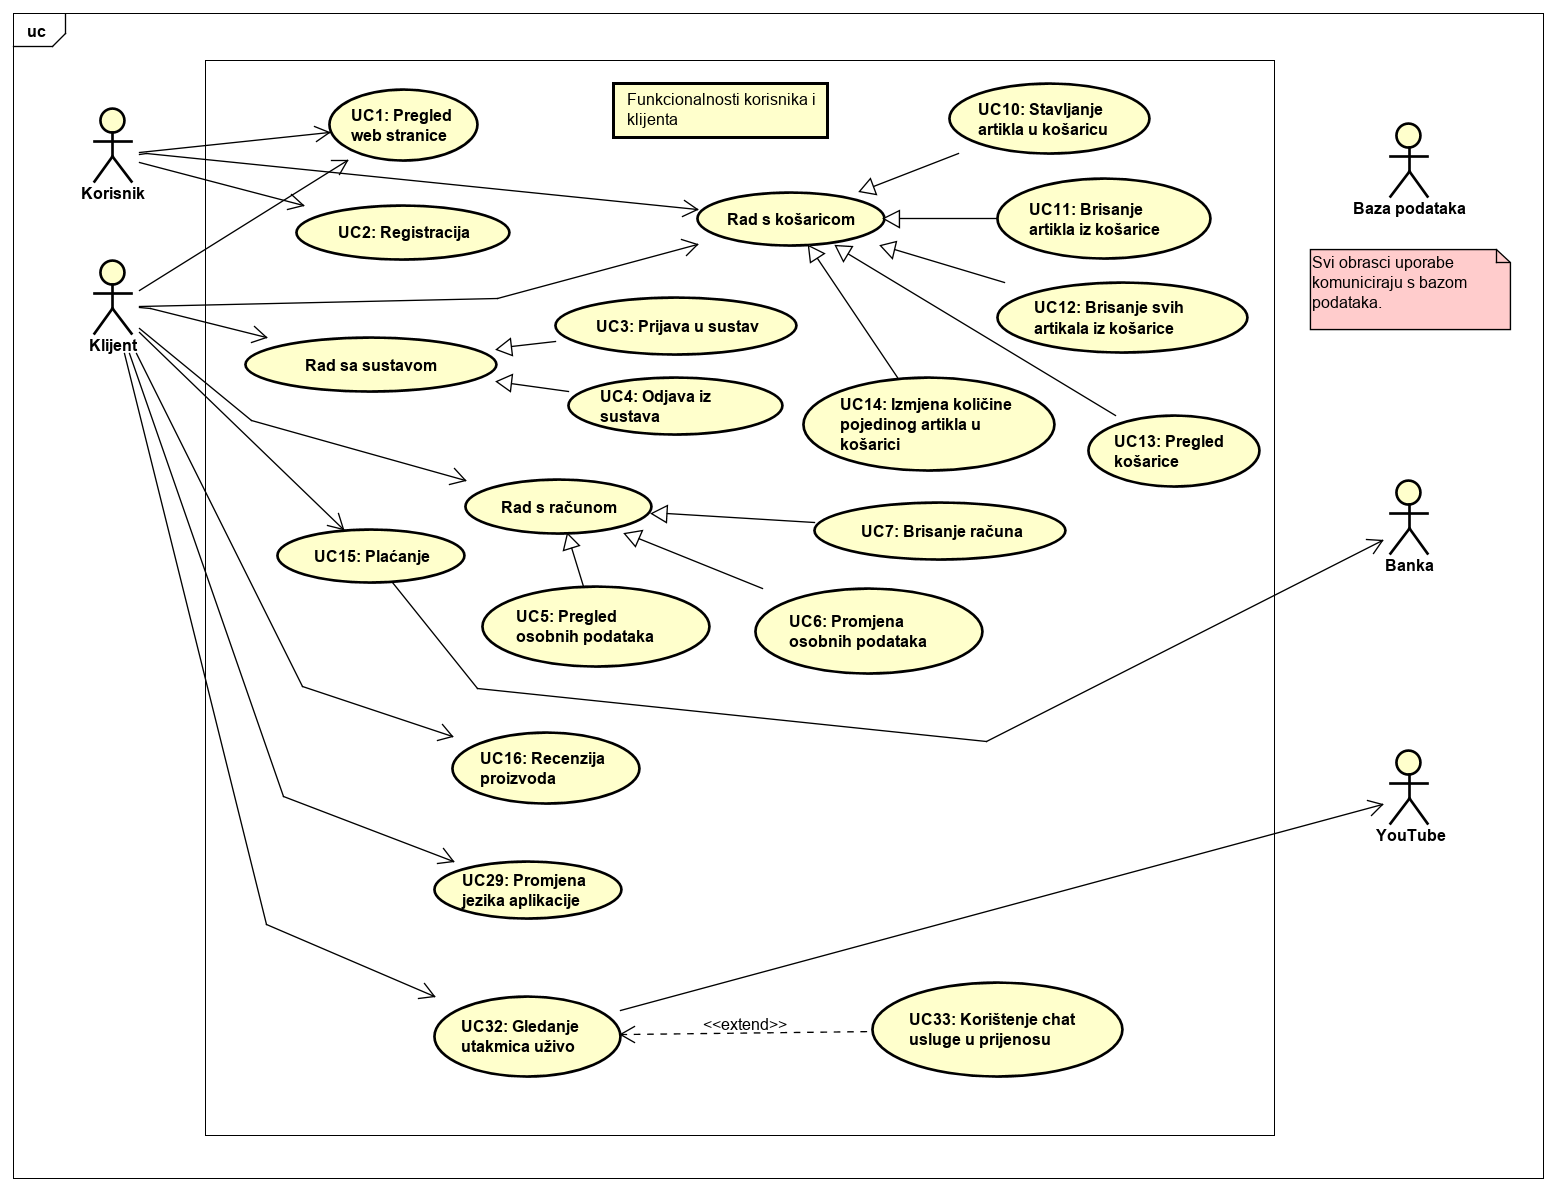
\includegraphics[scale=0.4]{dijagrami/Funkcionalnosti_korisnika_i_klijenta.png}
						\centering
						\caption{Funkcionalnosti korisnika i klijenta}
						\label{fig:UseCaseDiagram1}
					\end{figure}
				
					\begin{figure}[H]
						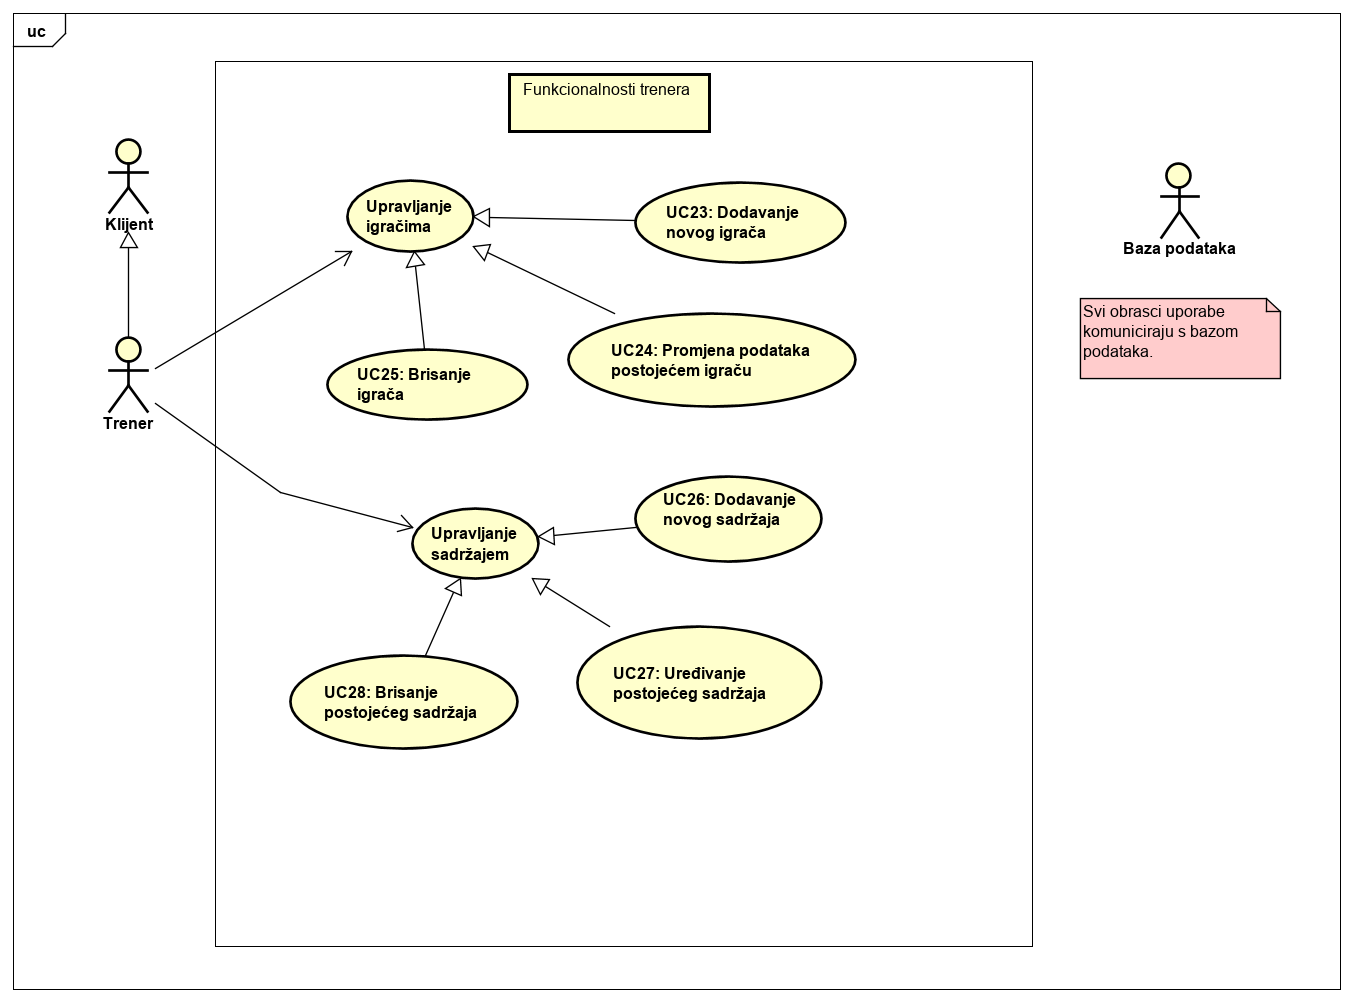
\includegraphics[scale=0.4]{dijagrami/Funkcionalnosti_trenera.png}
						\centering
						\caption{Funkcionalnosti trenera}
						\label{fig:UseCaseDiagram2}
					\end{figure}
				
					\begin{figure}[H]
						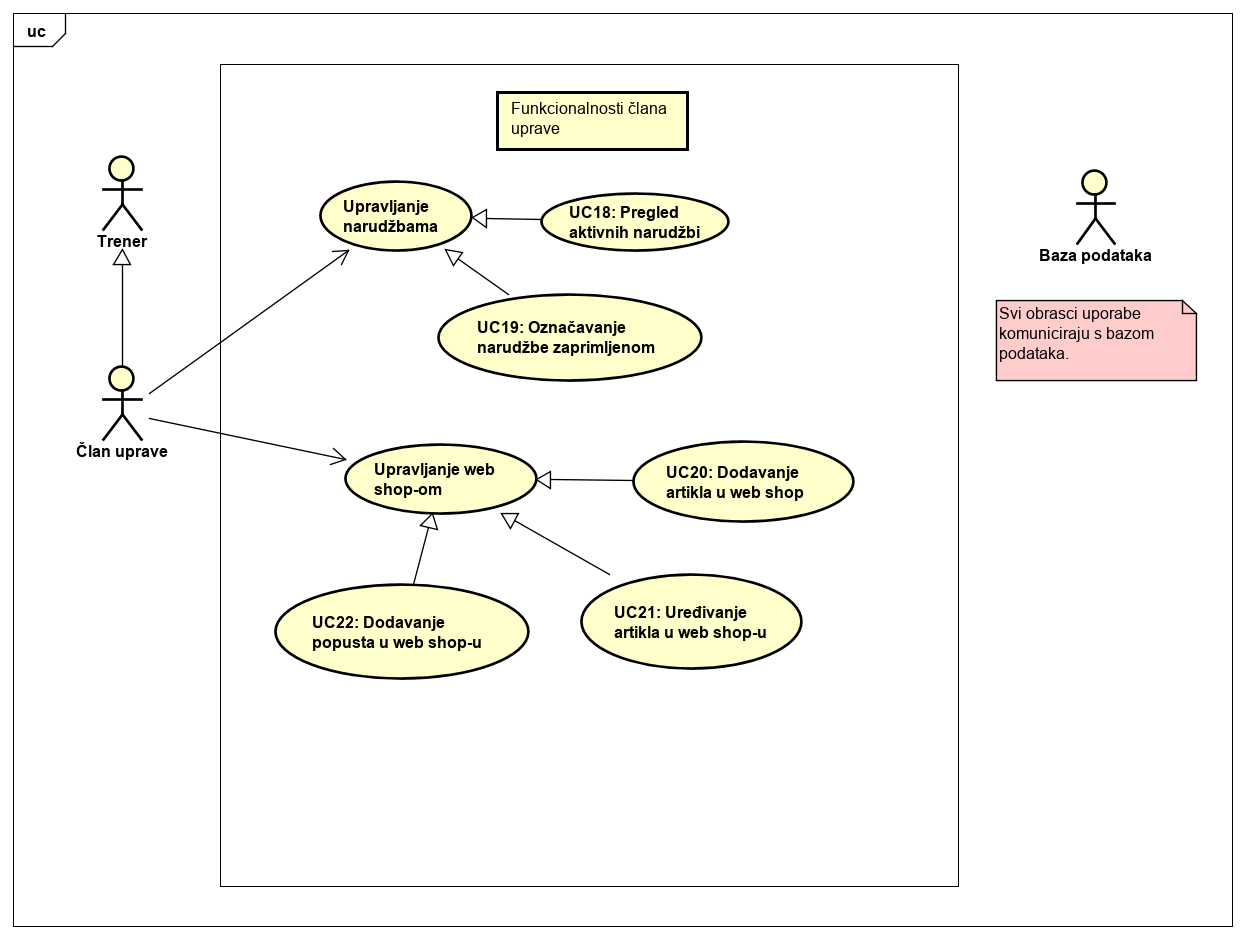
\includegraphics[scale=0.4]{dijagrami/Funkcionalnosti_clana_uprave.png}
						\centering
						\caption{Funkcionalnosti člana uprave}
						\label{fig:UseCaseDiagram3}
					\end{figure}
				
					\begin{figure}[H]
						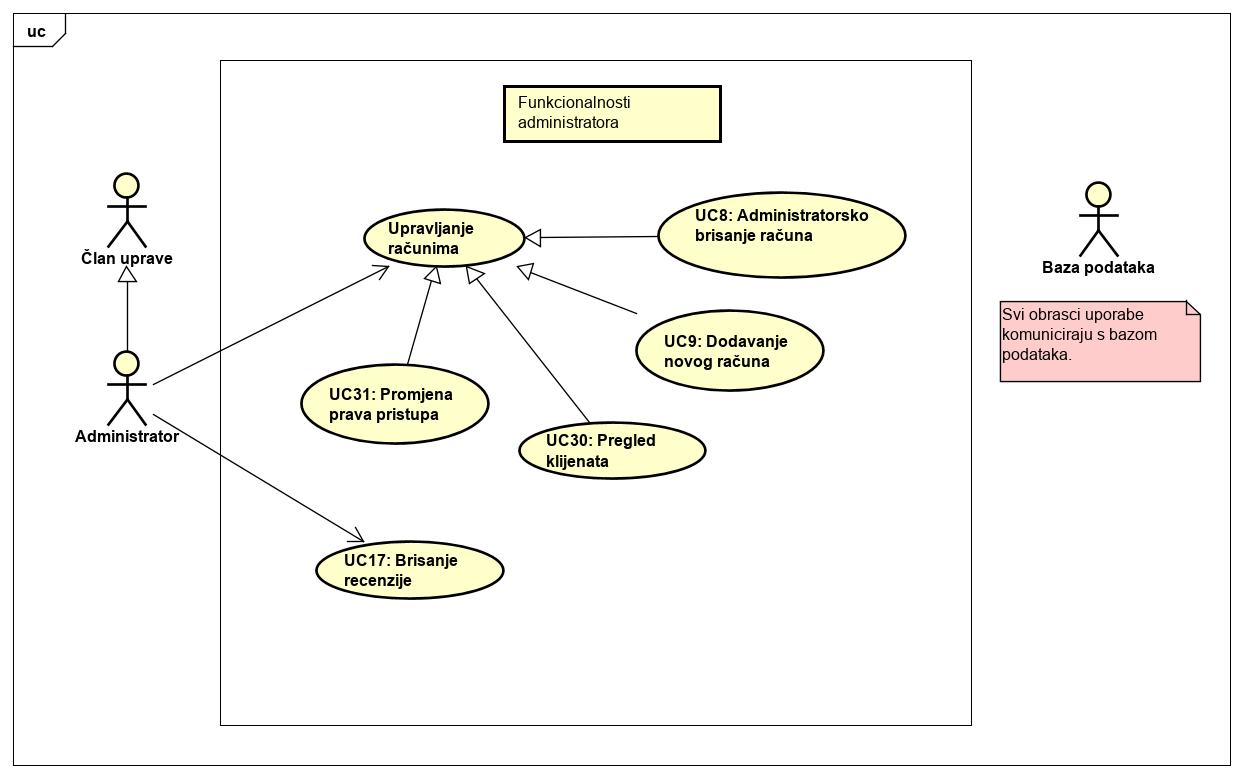
\includegraphics[scale=0.4]{dijagrami/Funkcionalnosti_administratora.png}
						\centering
						\caption{Funkcionalnosti administratora}
						\label{fig:UseCaseDiagram4}
					\end{figure}
				
				\eject		
				
			\subsection{Sekvencijski dijagrami}
				
				\textbf{\textit{dio 1. revizije}}\\
				
				\textit{Nacrtati sekvencijske dijagrame koji modeliraju najvažnije dijelove sustava (max. 4 dijagrama). Ukoliko postoji nedoumica oko odabira, razjasniti s asistentom. Uz svaki dijagram napisati detaljni opis dijagrama.}
				\eject
				
				\begin{figure}[H]
					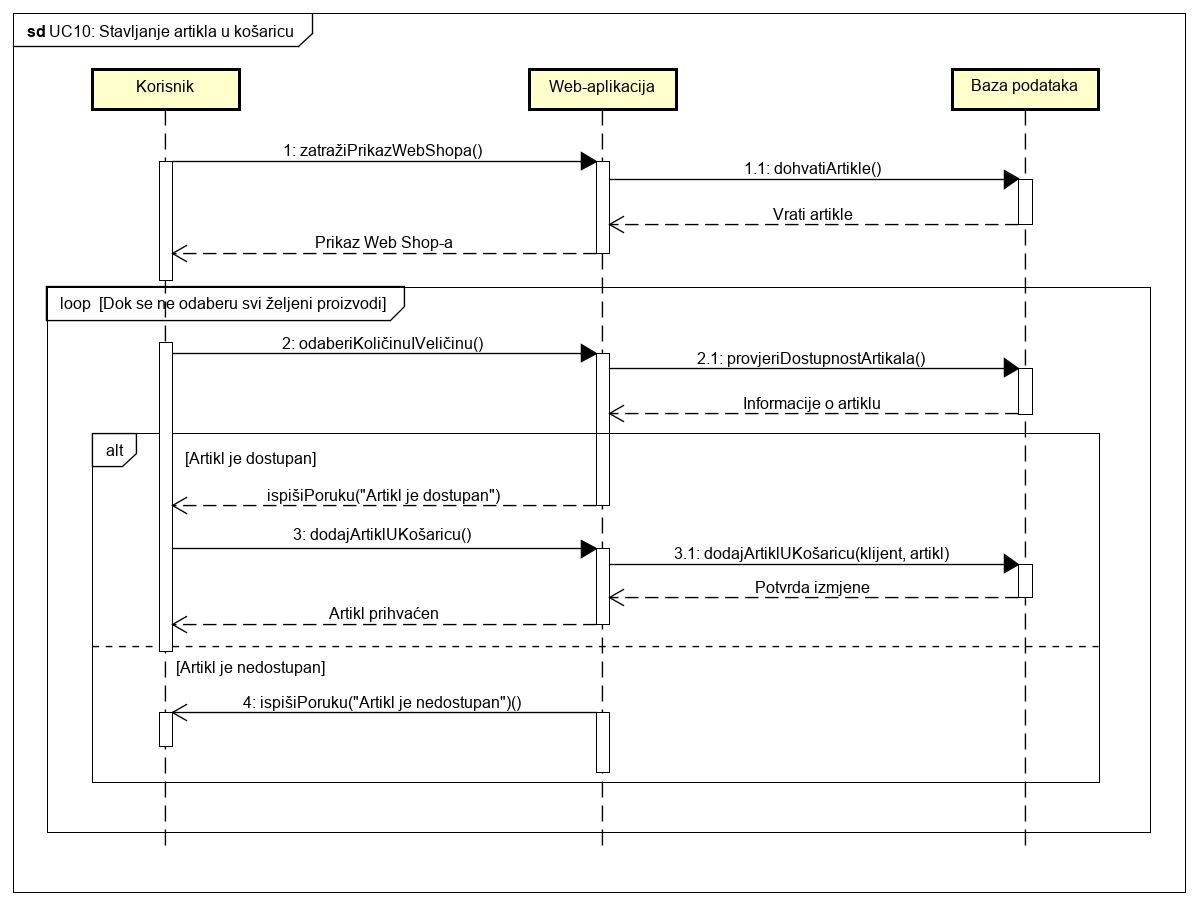
\includegraphics[scale=0.4]{dijagrami/UC10.png}
					\centering
					\caption{UC10, Stavljanje artikla u košaricu}
					\label{fig:SequanceDiagram1}
				\end{figure}
			
				\begin{figure}[H]
					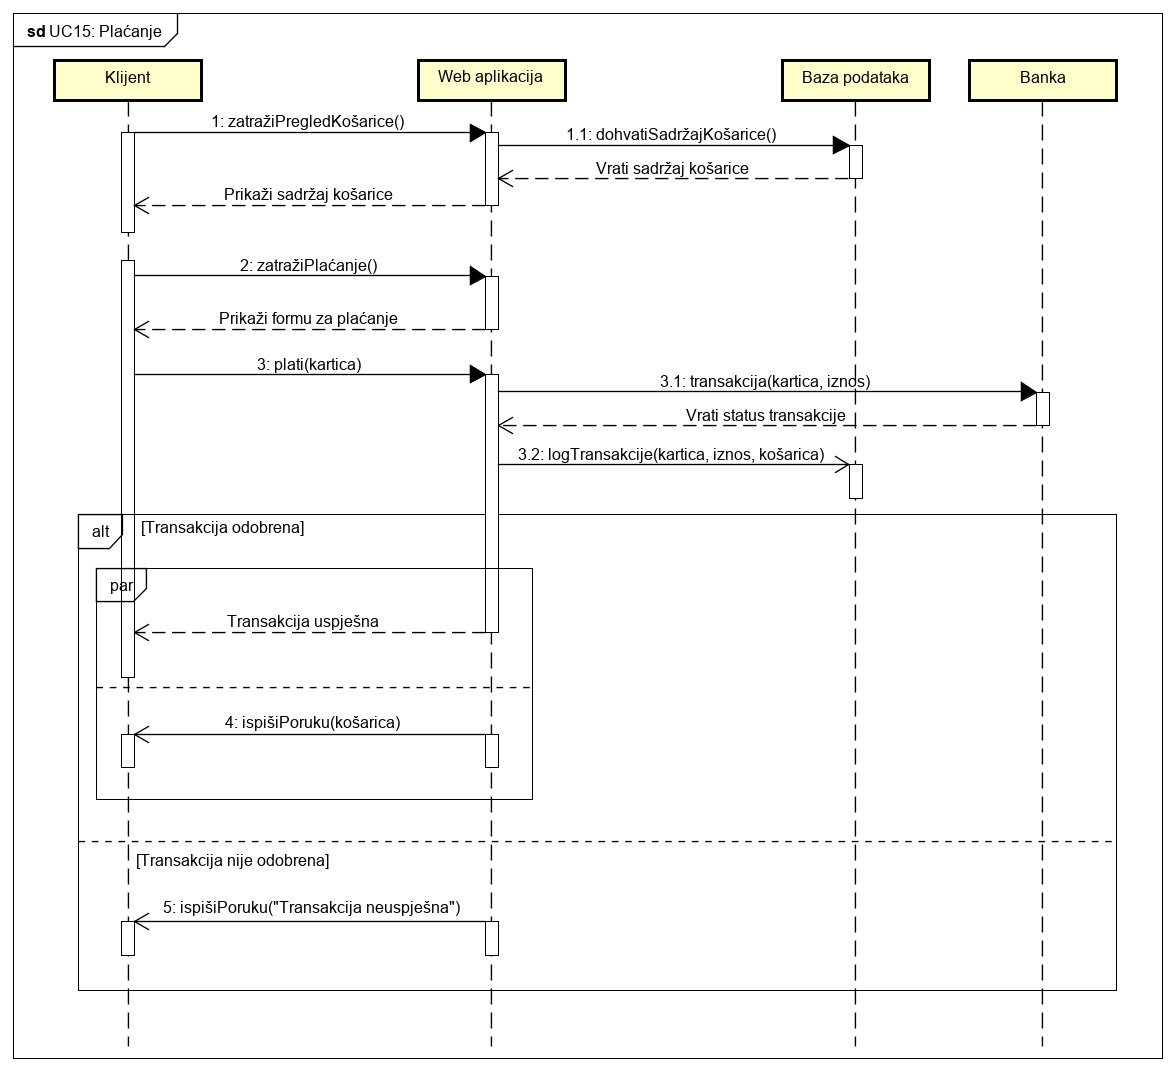
\includegraphics[scale=0.4]{dijagrami/UC15.png}
					\centering
					\caption{UC15, Plaćanje}
					\label{fig:SequanceDiagram2}
				\end{figure}
			
				\begin{figure}[H]
					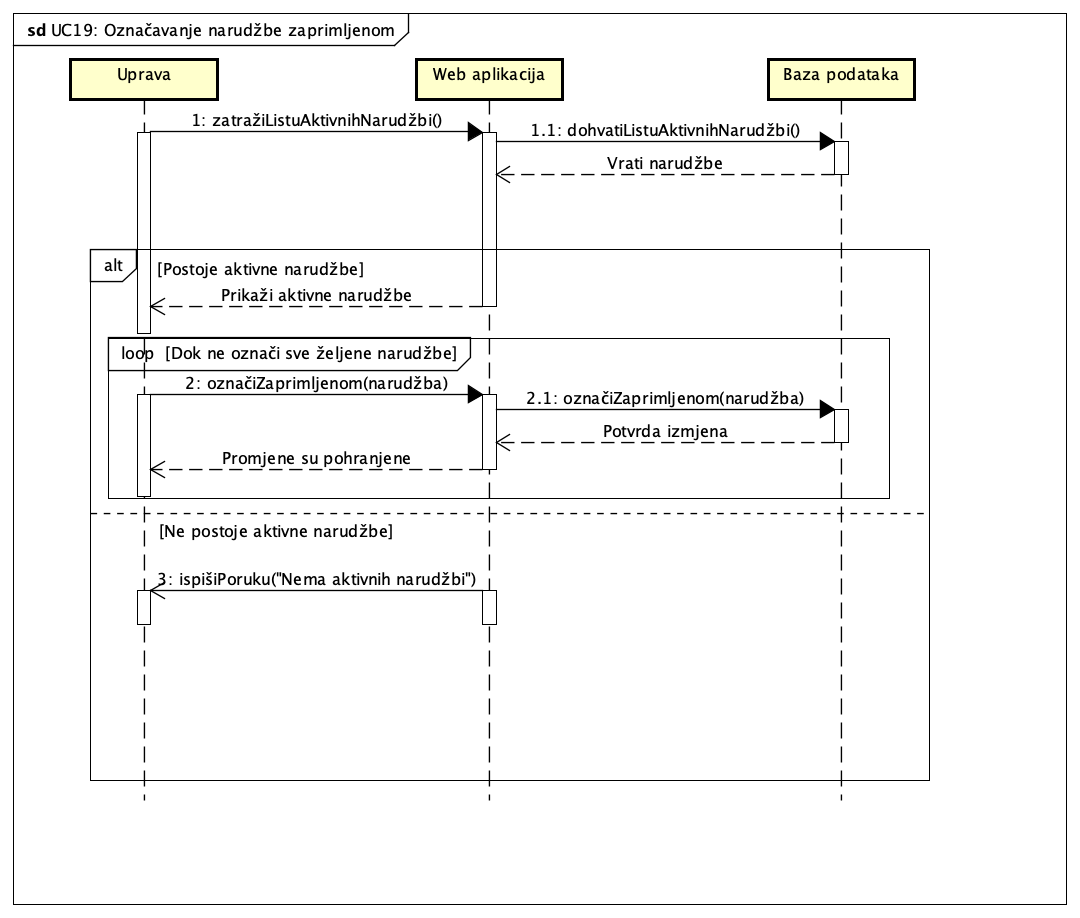
\includegraphics[scale=0.4]{dijagrami/UC19.png}
					\centering
					\caption{UC19, Označavanje narudžbe gotovom}
					\label{fig:SequanceDiagram3}
				\end{figure}
			
				\begin{figure}[H]
					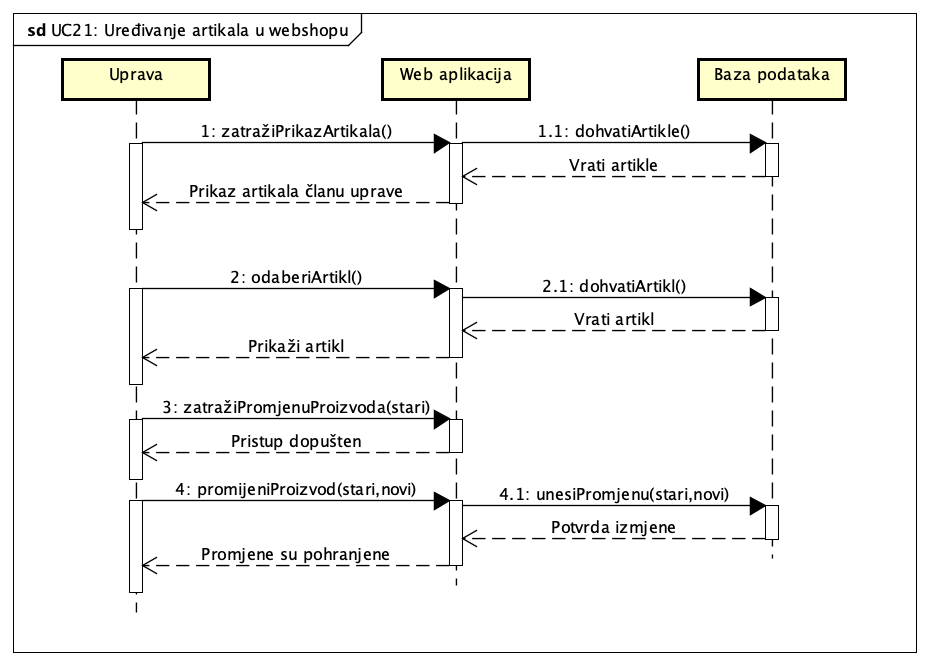
\includegraphics[scale=0.4]{dijagrami/UC21.png}
					\centering
					\caption{UC21, Uređivanje artikala u web shopu}
					\label{fig:SequanceDiagram4}
				\end{figure}
	
		\section{Ostali zahtjevi}
		
			\begin{packed_item}
				\item Sustav treba omogućiti rad više korisnika u stvarnom vremenu
				\item Korisničko sučelje i sustav moraju podržavati hrvatsku abecedu (dijakritičke znakove) pri unosu i prikazu tekstualnog sadržaja
				\item Izvršavanje dijela programa u kojem se pristupa bazi podataka ne smije trajati duže od nekoliko sekundi
				\item Sustav treba biti implementiran kao web aplikacija koristeći objektno-orijentirane jezike
				\item Neispravno korištenje korisničkog sučelja ne smije narušiti funkcionalnost i rad sustava
				\item Sustav treba biti jednostavan za korištenje, korisnici se moraju znati koristiti sučeljem bez opširnih uputa
				\item Nadogradnja sustava ne smije narušavati postojeće funkcionalnosti sustava
				\item Sustav kao valutu koristi HRK
				\item Veza s bazom podataka mora biti kvalitetno zaštićena, brza i otporna na vanjske greške
				\item Front-end web aplikacije bit će implementiran uz pomoć HTML5, CSS3, Bootstrap 4 i Vue.js tehnologija
				\item Back-end web aplikacije bit će implementiran u programskom jeziku C\#
				\item Čitav sustav će biti utemeljen na okviru rada ASP.NET Core 3.0
				\item Sustav će podržavati hrvatski i engleski jezik
			\end{packed_item}

			 
			 
			 
	